\section{The Model for a Personalized HIV Treatment}
\label{sec:model}

In this section, we introduce a mathematical model that allows us to simulate the evolution of an HIV infection.
After further investigating this model and discussing the impact of antiretroviral drugs, the optimal control problem is formulated.

\subsection{The Dynamic Model}
\label{subsec:Model_DynModel}

Since HIV was first simulated in the mid-90s, a wide variety of different models arose.
Initially, they attempted to investigate the HIV evolution by a set of linear \textit{ordinary differential 
equations} (ODEs). These, however, are only applicable for a short period of time, ranging in the orders of days.
HIV, treated or untreated, is a disease that lasts for years, and accurate and reliable long-term investigations 
require non-linear models \cite{adams2005hiv}.\newline
In addition hereto, the final model definition is determined by the choice of biological compartments and interactions 
that one wants to simulate.
Some models, for instance, differentiate between potential target cells, usually including CD4+ T cells and macrophages \cite{perelson1993dynamics}.
Once a cell is infected, it can either remain in a latent state or actively reproduce new viral cells, causing different reactions of 
the patient’s immune system \cite{anderson1998complex}.\par

\begin{figure}
    \centering
    \begin{subfigure}[b]{0.3\textwidth}
        \centering
        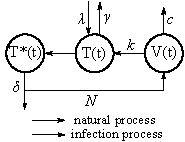
\includegraphics[width=0.75\textwidth]{images/infection_scheme/untreated_infection.pdf}
        \caption[]%
        {{\small Dynamics of untreated HIV infection}}    
        \label{fig0a:scheme_pretreatment}
    \end{subfigure}
    \begin{subfigure}[b]{0.625\textwidth}   
        \centering 
        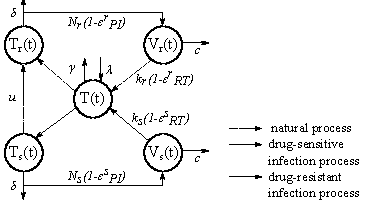
\includegraphics[width=0.7\textwidth]{images/infection_scheme/treated_infection.pdf}
        \caption[]%
        {{\small Dynamic of HIV infection under HAART}}    
        \label{fig0b:scheme_treated}
    \end{subfigure}
    \caption[]{The above diagrams visualise two scenarios of an HIV infection.
    Model (a) describes the evolution of an untreated infection by distiguishing between uninfected target cells $T(t)$, infected ones $T^*(t)$ and viral cells $V(t)$.
    A healthy body strives to maintain a constantly high number of CD4+ T cells.
    While these cells die at the end of their life span with frequency $\gamma$, the human immune system continuously produces new ones at a birth rate $\lambda$.
    However, under the impact of HIV, the number of immune cells $T(t)$ is not only reduced by natural death but also due to the virus.
    First, CD4+ T cells are infected at rate $k$ and the viral genetic material is included in their cellular DNA.
    During the remaining life time, the infected cell replicates the viral genes until it finally bursts, described by the bursting rate $\delta$, and releases $N$ new viral cells.
    Some of these, again, start infecting healthy CD4+ T cells while the rest die before they find a host cell which they can exploit to multiply their viral genes.
    Parameter $c$ describes the death rate of viral cells.
    Opposed to that, model (b) explains the dynamics of a treated HIV infection, taking arising drug-resistant virus mutations into account.
    Although, the principle of the infection cycle remains the same, the extended model now differentiates between two cocirculating populations of cells: the ones which are susceptible to drugs, i.e. $V_s(t)$ and $T_s(t)$ as well as those that aren't, described by $V_r(t)$ and $T_r(t)$.
    Drug-resistant virus cells lead to infected cells which solely reproduce further resistant viruses.
    % The only transition between the two populations can be observed during replication.
    In contrast hereto, in a CD4+ T cell which is infected by a drug-sensitive virus, the HIV genome might mutates during replication and becomes resistant.
    Additionally, the diagram illustartes the effect of HAARTs.
    Tabel \ref{tab:init_parameters} summarises the meaning of the used parameters.
    % The RTIs reduce the infection rate of the virus while the effect of PIs first comes in after the infected cells bursted.
    % A smaller number of released viral cells can participate in the next round of infection.\par
    }
    \label{fig:infection_schemes}
\end{figure}

% Scheme \ref{fig0a:scheme_pretreatment}, for instance, visualises the mechanisms of an untreated HIV infection.
A simple model, for instance, is shown in figure \ref{fig0a:scheme_pretreatment}.
It describes the evolution of an HIV infection, assuming that no thearpy measures are taken.
% To understand the basic dynamics it suffices to distiguish between uninfected target cells, infected ones and viral cells.
% A healthy body strives to maintain a constant number of CD4+ T cells.
% While these cells die at the end of their life span, the human immune system continuously produces new ones at a constant birth rate.
% However, under the impact of HIV, the number of immune cells is not only reduced by natural death but also due to the virus.
% First, CD4+ T cells are infected and the viral genetic material is included in their cellular DNA.
% During the remaining life time, the infected cell replicates the viral genes until it finally bursts and releases multiple new viral cells.
% Some of these, again, start infecting healthy CD4+ T cells while the rest die before they find a host cell which they can exploit to multiply their viral genes.\par
However, to optimize HAARTs, we have to further evolve this model in order to not only simulate the interaction between viral and immune cells but 
to also consider the effect of drugs.
% To optimize HAARTs, we require a model that does not only simulate the interaction between viral and immune cells but 
% one that also considers the effect of the taken drugs.\newline
For this, we first have to review the working principle and impact of HAART.
Generally, this therapy is a combination of multiple classes of antiretroviral drugs, each fighting the virus in different ways.
Two of these are \textit{reverse transcriptase inhibitors} (RTIs) and \textit{protease inhibitors} (PIs).
While the first aims at blocking the initial infection of target cells, the latter causes already infected cells to only produce 
immature virus.
Both these drugs, are solely designed for virus cells with a specific genome.
HIV, however, replicates in untreated persons at an exponentional rate, generating up to $10^{10}$ new free virus 
cells per day. Essential steps in this duplication are error-prone and hence, the probability of mutations is high.
The emerging cells have modified genomes, and the deployed drugs inhibt them less efficiently.
Thus, an appropriate model has to distiguish between drug-sensitive and resistant viruses \cite{rong2007emergence}.
Such a model is shown in figure \ref{fig0b:scheme_treated}.\newline
% Although, the principle of the infection cycle remains the same, the extended model now differentiates between two cocirculating populations of target and viral cells: the ones which are susceptible to drugs and those that aren't.
% Drug-resistant virus cells lead to infected cells which solely reproduce further resistant viruses.
% % The only transition between the two populations can be observed during replication.
% In contrast hereto, in a CD4+ T cells which is infected by a drug-sensitive virus, the HIV genome might mutates during replication and becomes resistant.
% Additionally, the diagram illustartes the previously described effect of HAARTs.
% % The RTIs reduce the infection rate of the virus while the effect of PIs first comes in after the infected cells bursted.
% % A smaller number of released viral cells can participate in the next round of infection.\par

According Rong et al. \cite{rong2007emergence}, the dynamics in figure \ref{fig0b:scheme_treated}, can be described by the following set 
of differential equations:

\begin{align}
    \begin{split}
        \dot{T}(t) &= \lambda - \gamma T(t) - k_s (1 - \varepsilon_{RT}^s) V_s(t) T(t) - k_r (1 - \varepsilon_{RT}^r) V_r(t) T(t),\\
        \dot{T_s}(t) &= (1-u)k_s(1 - \varepsilon_{RT}^s)V_s(t)T(t) - \delta T_s(t),\\
        \dot{V_s}(t) &= N_s \delta (1 - \varepsilon_{PI}^s) T_s(t) - c V_s(t),\\
        \dot{T_r}(t) &= u k_s (1 - \varepsilon_{RT}^s) V_s(t) T(t) + k_r (1 - \varepsilon_{RT}^r) V_r(t) T(t) - \delta T_r(t),\\
        \dot{V_r}(t) &= N_r (1 - \varepsilon_{PI}^r) \delta T_r(t) - c V_r(t).
    \end{split}
    \label{equ:HIVmodel}
\end{align}

Here, $T(t)$ denotes the concentration of uninfected target T cells.
Generally, by index $s$ we denote the drug-sensitive strain whereas index $r$ marks the drug-resistant one.
% As discussed above, we are distiguishing between drug sensitive and resistant strains.
Thus, $T_s(t)$ is the concentration of cells that are infected by drug-sensitive viral cells $V_s(t)$, whereas $T_r(t)$ is the concentration of cells that are infected by drug-resistant viral cells $V_r(t)$.
All concentrations are given in $1/ml$.
Note, that the five compartments in model \ref{equ:HIVmodel} are not directly observable in clinical data.
Instead, blood measurements only give insight into the total viral load, i.e. $V_{tot}(t) = V_r(t) + V_s(t)$ and the overall number of 
immune cells, given as $T_{tot}(t) = T(t) + T_r(t) + T_s(t)$.\newline
Further, $\lambda$ represents the birth rate of uninfected T cells per day, $\gamma$ is their per capita daily death rate.
% Apart from natural death, the T cell population is reduced by infection. 
The constant rates $k_s$ and $k_r$ describe how fast uninfected cells are infected by drug-sensitive and resistant virus, respectively.
At the same time, these rates are reduced by the use of RITs. The efficacy of the drug is given by the dimensionless 
parameters $\varepsilon_{RT}^{s}$ and $\varepsilon_{RT}^{r}$, both ranging between 0 and 1.
Since sensitive viruses are more susceptible to drugs, $\varepsilon_{RT}^{s} > \varepsilon_{RT}^{r}$.\newline
We assume that both kinds of infected cells, $T_s(t)$ and $T_r(t)$, burst and consequently die at the same daily rate $\delta$.
% During bursting, a certain number of free virus cells are released. 
For sensitive virus cells, the number of released virus cells is denoted by $N_s$ 
while $N_r$ describes the same quantitiy in the drug-resistant case.
However, under the deployment of PIs, not all of the newly generated free virus cells are themselves capable of infecting healthy immune 
cells. This is encoded in the efficacy parameters $\varepsilon_{PI}^s$ and $\varepsilon_{PI}^r$. Again, $0 \leq \varepsilon_{PI}^s \leq 1$, 
$0 \leq \varepsilon_{PI}^r \leq 1$ and $\varepsilon_{PI}^s > \varepsilon_{PI}^r$.
Virus cell populations are only reduced by their daily clearance rate $c$.\newline
With the parameters $\varepsilon_{RT}$ and $\varepsilon_{PI}$, we describe the efficacy of the single antiretroviral drugs.
Summarizing these to the overall drug efficacy $\varepsilon = 1 - (1-\varepsilon_{RT})(1-\varepsilon_{PI})$ allows us to assess the efficacy of 
the combination therapy.
Hence,

\begin{align}
    \begin{split}
        \varepsilon_s &= 1 - (1-\varepsilon_{RT}^s)(1-\varepsilon_{PI}^s)\, ,\\
        \varepsilon_r &= 1 - (1-\varepsilon_{RT}^r)(1-\varepsilon_{PI}^r) \,\text{.}
    \end{split}
    \label{equ:epsilon_HAART}
\end{align}

Drug efficacy $\varepsilon_s$ only depends on the current therapy can directly be derived from drug dosages and intake durations.
At the same time, we assume that the resistance level of the HIV mutants can be quantified by the parameter $\alpha\; (0 < \alpha < 1)$, 
which represents the reduction in drug effectiveness by $\varepsilon_{RT}^s = \alpha \varepsilon_{RT}^r$ and $\varepsilon_{PI}^s = \alpha \varepsilon_{PI}^r$.
Additionally, the rate at which $T_s(t)$ cells become drug-resistant during the process of replication is given by the parameter $u$ ($0 \leq u < 1$).
In this chapter, we assume mild mutations, i.e. they appear rather seldomly and if they do, their susceptibility is only little reduced.
Mathematically, this behaviour is achieved by setting $u = 3 \times 10^{-5}$ and $\alpha = 0.2$.
With that, the efficacy parameters in relation \ref{equ:epsilon_HAART} are known and constant.\newline
Opposed to that, the remaining parameters, summarized in $\vec{\theta} = \{\lambda, \gamma, k_s, k_r, N_s, N_r, \delta, c\}$, strongly depend on the patient.
With the given information about the therapy, they can be estimated from blood measurements.
Descriptions and units of all parameters are summarized in table \ref{tab:init_parameters}.\par

\renewcommand{\arraystretch}{1.25}
\begin{table}
    \centering
    % \begin{tabular}{m{5em} m{10em} m{20em}}
        \begin{tabular}{ ccc }
        \hline
        \hline
        % \multicolumn{3}{c}{\textit{Parameter definitions and values used in numerical simulation}} \\
        % \hline
        % \rule{0pt}{10pt}
        Parameter & Value & Description\\[0.5ex]
        \hline
        $\lambda$   & $10^4\,\text{ml}^{-1}\text{day}^{-1}$ (estimated)& Birth rate of uninfected cells\\
        $\gamma$   & $0.01\,\text{day}^{-1}$  (estimated)& Natural death rate of uninfected cells\\
        $k_s$   & $2.4 \times 10^{-8}\,\text{ml}\,\text{day}^{-1}$  (estimated)& Infection rate of target cells by drug-sensitive virus\\
        $k_r$   & $2.0 \times 10^{-8}\,\text{ml}\,\text{day}^{-1}$  (estimated)& Infection rate of target cells by drug-resistant virus\\
        $u$   & $3 \times 10^{-5}$  (given)& Mutation rate from sensitive to resistant strain\\
        $\delta$   & $1\,\text{day}^{-1}$  (estimated)& Death rate of infected cells\\
        $N_s$   & $3000$ (estimated)& Burst size of drug-sensitive strain\\
        $N_r$   & $2000$ (estimated)& Burst size of drug-resistant strain\\
        $c$   & $23\, \text{day}^{-1}$  (estimated)& Clearance rate of free virus\\
        $\varepsilon_{RT}^{s}$  & varies (given)& Efficacy of RTIs for sensitive strain\\
        $\varepsilon_{RT}^{r}$  & varies (given)& Efficacy of RTIs for resistant strain\\
        $\varepsilon_{PI}^{s}$  & varies (given)& Efficacy of PIs for sensitive strain\\
        $\varepsilon_{PI}^{r}$  & varies (given)& Efficacy of PIs for resistant strain\\
        $\varepsilon_{s}$  & varies (given)& Overall drug efficacy for sensitive strain\\
        $\varepsilon_{r}$  & varies (given)& Overall drug efficacy for resistant strain\\
        $\alpha$  & varies (given)& Resistance level of mutant strain\\
        \hline
        \hline
    \end{tabular}
    \caption{The tabel gives an overview about the model parameters, their definitions and physical units.
    The listed values, which are used for the numerical simulations to investigate the model, are based on a paper by Rong et al. \cite{rong2007emergence}.}
    \label{tab:init_parameters}
\end{table}

% The final objective is to derive model parameters from the clinical data of one patient, and hence explicitly tailor it to that person.
% However, before doing so, we are examining the model itself in more detail.
Before tailoring the above model \ref{equ:HIVmodel} to a specific patient, its dynamic and steady state behaviour is validated by comparing numerical results 
to clinical observations and findings from research.
In addition hereto, such simulations give deeper insight into the impact of antiretroviral drugs.
If not stated differently, parameters are taken from table \ref{tab:init_parameters}.\newline
Firstly, we consider a pretreatment situtaion.
A patient, who has been healthy until the very day of infection, has a CD4+ T cell count of $T(0) = 10^{6} \, \text{ml}^{-1}$.
If she or he is infected by a viral load of $V_s(0) = 10^{-6} \, \text{ml}^{-1}$, the untreated virus (i.e. $\varepsilon_s = \varepsilon_r = 0$) 
evolves within the first weeks as depicted in figure \ref{fig:untreated}.
Note, that although the transmitted pathogens could have already been mutated, it is assumed that $V_r(0) = 0\, \text{ml}^{-1}$.
The further inital values are set to $0$ \cite{perelson1993dynamics}.\newline
From figure \ref{fig:untreated} it can be seen, that the dynamic characteristics of the model coincide with the previously described stages
of an untreated HIV infection.
While in the first few weeks, the viral load increases strongly, the number of uninfected T cells collapses, resulting in often observed flu-like 
symptomes. 
% This phase is often accompanied by strong symptoms, resembling a flu.
Following this, the model shows how the state of clinical latency sets in.
Here, the viral loads as well as $T$ settle in a steady state.
Figure \ref{fig1c:viral_load} demonstrates that without medication, the drug-sensitive strain dominates the infection throughout the 
considered time interval.

\begin{figure}
    \centering
    \begin{subfigure}[b]{0.475\textwidth}
        \centering
        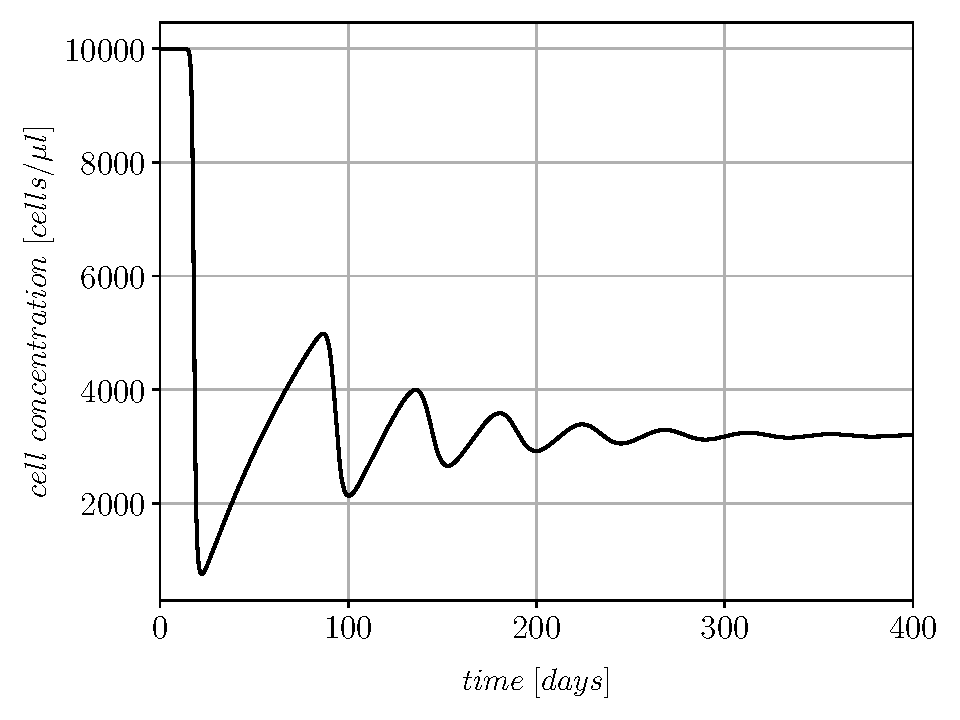
\includegraphics[width=\textwidth]{images/eRT_0_alpha_0/untreated_T.pdf}
        \caption[]%
        {{\small Uninfected CD4+ T cells}}    
        \label{fig1a:uninfected_T_cells}
    \end{subfigure}
    \begin{subfigure}[b]{0.475\textwidth}   
        \centering 
        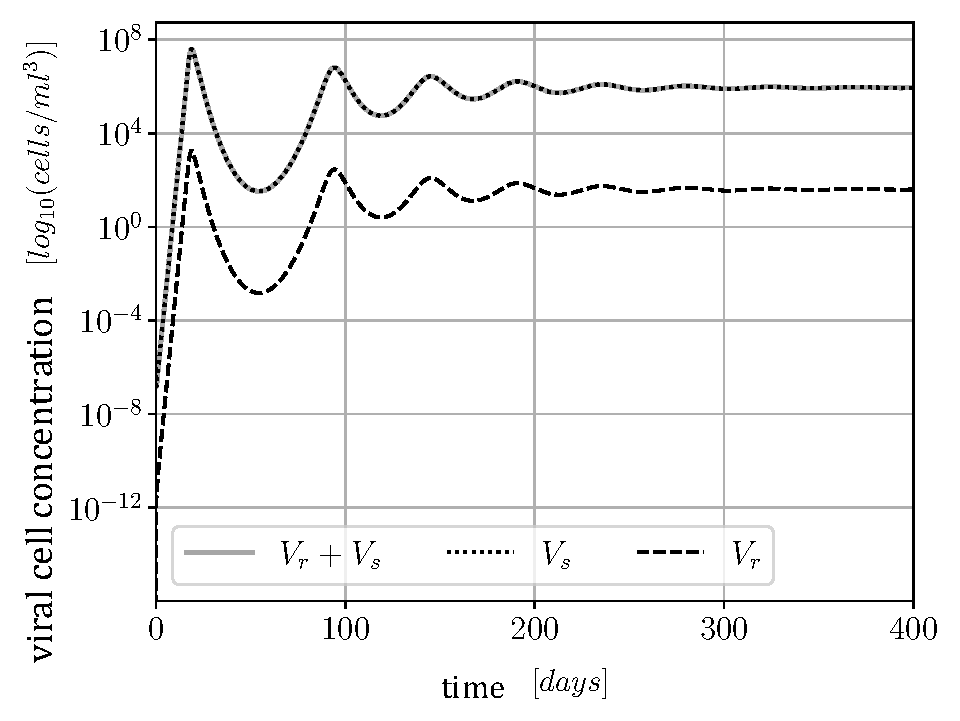
\includegraphics[width=\textwidth]{images/eRT_0_alpha_0/untreated_overview_V.pdf}
        \caption[]%
        {{\small Viral load}}    
        \label{fig1c:viral_load}
    \end{subfigure}
    \caption[]{Simulation of the pretreatment evolution of an initial HIV infection.
    For the inital state, the following values are assumed: $T(0) = 10^{6} \, \text{ml}^{-1}$, $T_s(0) = 0 \, \text{ml}^{-1}$, 
    $T_r(0) = 0 \, \text{ml}^{-1}$, $V_s(0) = 10^{-6} \, \text{ml}^{-1}$ and $V_r(0) = 0 \, \text{ml}^{-1}$ \cite{perelson1993dynamics}.
    Diagram (a) describes evolution of the uninfected CD4+ T cells during the first year.
    After an inital break-in of $T(t)$, which is followed by oscillations, the immune cell concentration finally settles at a low level.
    At the same time, the total number of viral cells, i.e. $V_r(t) + V_s(t)$ increases.
    This behaviour is shown in figure (b), where the concentrations of the total viral load as well as its two strains $V_r(t)$ and $V_s(t)$, is plotted in a semi-logarithmic scale.
    Similar to the immune cells, the concentrations of the virus exhibits oscillations, before it remains roughly constant.}
    \label{fig:untreated}
\end{figure}

We assume that at this point of the disease, the infection is recognized and HAART is prescribed.
With a presumed low resistance level of $\alpha = 0.2$, the therapy is quantified by $\varepsilon_{RT}^{s} = 0.4$ and $\varepsilon_{PI}^{s} = \varepsilon_{PI}^{r} = 0$.
As initial values, the steady states of the pretreatment simualtion are chosen.\newline
The numerical results, given in figure \ref{fig2:treated_eRT_04_alpha_02}, show that indeed the therapy lowers the viral load and allows the 
number of uninfected immune cells to rise again.

\begin{figure}
    \centering
    \begin{subfigure}[b]{0.475\textwidth}
        \centering
        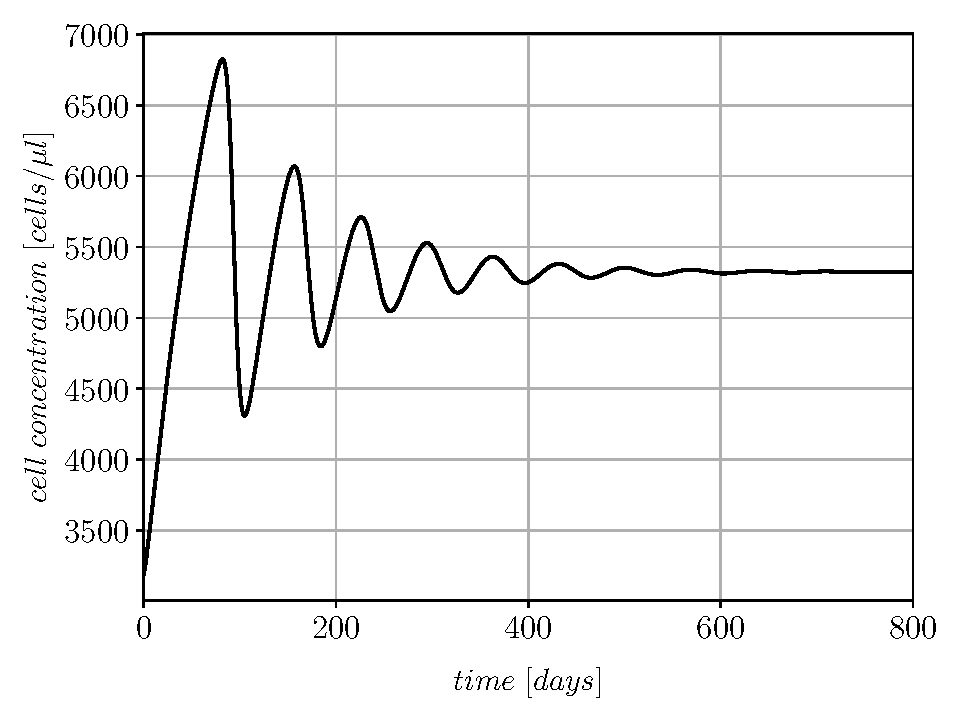
\includegraphics[width=\textwidth]{images/eRT_04_alpha_02/treated_T.pdf}
        \caption[]%
        {{\small Uninfected CD4+ T cells}}    
        \label{fig2a:uninfected_T_cells}
    \end{subfigure}
    \begin{subfigure}[b]{0.475\textwidth}   
        \centering 
        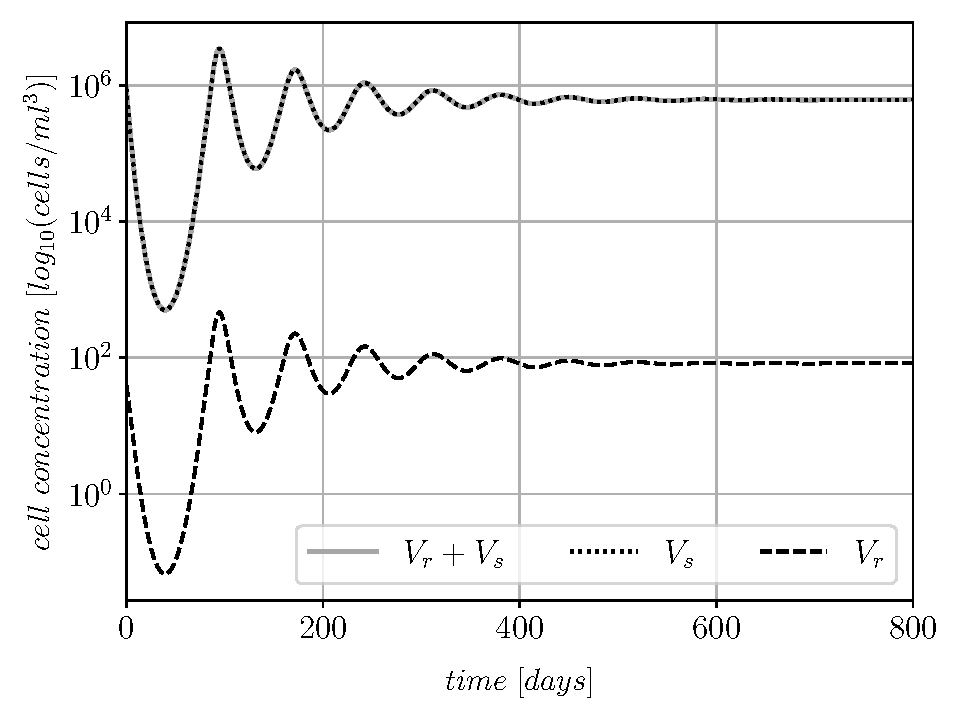
\includegraphics[width=\textwidth]{images/eRT_04_alpha_02/treated_overview_V.pdf}
        \caption[]%
        {{\small Viral load}}    
        \label{fig2c:viral_load}
    \end{subfigure}
    \caption[]{Simulation of the evolution of an HIV infection under HAART.
    It is $\varepsilon_{RT}^s = 0.4$, $\varepsilon_{RT}^r = \alpha \varepsilon_{RT}^s$ with $\alpha = 0.2$ and 
    $\varepsilon_{PI}^s = \varepsilon_{PI}^r = 0$.
    The steady states of the preceding pretreatment simulation are used as initial values, i.e. $T(0) = 3.19 \times 10^{5} \, \text{ml}^{-1}$, 
    $T_s(0) = 6.81 \times 10^{3} \, \text{ml}^{-1}$, $T_r(0) = 0.46 \, \text{ml}^{-1}$, $V_s(0) = 8.88 \times 10^{5} \, \text{ml}^{-1}$ 
    and $V_r(0) = 39.95 \, \text{ml}^{-1}$ \cite{perelson1993dynamics}.
    Diagram (a) shows the evolution of the CD4+ T cell count during the first two years of therapy.
    Similar can be seen in diagram (b), where the concentration of the viral load is depicted on a semi-logarithmic scale.
    Immune and viral cells are in a constant competition.
    Initially, therapy surpresses the reproduction of viral cells and hence, their concentration rapidly sinks.
    Consequently, more uninfected T cells are produces and $T(t)$ peaks in that first therapy phase.
    At the same time, this increased number of potential host cells for the virus again fuels its replication, resulting in a growth of $V_r(t)$ and $V_s(t)$ increase again.
    Figure (a) and (b) exhibit this interplay in form of oscillations. 
    With time, this interaction settels at a constant level and the concentration of immune and viral cells remain roughly constant.
    Further, figure (b) gives insight into the behaviour of the two viral strains. Since we are assuming mild mutations which occure seldomly, the concentration of the drug resistant virus is remarkably smaller than $V_s(t)$.}
    \label{fig2:treated_eRT_04_alpha_02}
\end{figure}

An essential feature of the model is the development of the steady states as a function of medication efficacy of the drug-sensitive strain.
This is demonstrated in figure \ref{fig3:evolution_over_epsilon}, where the CD4+ T cell and viral count are plotted over $\varepsilon_s$.
From diagram \ref{fig3a:uninfected_T_cells}, it can be seen that for low values of $\varepsilon_s$, HAART achieve an increase in the 
number of uninfected target cells.
However, above a certain point, this growth saturates and the concentration remains on a constantly high level.
We denote this point of maximal efficacy by $\varepsilon_{s,max}$. 
For the given set of model parameters, its value is $\varepsilon_{s,max} \approx 0.5$.
A similar behaviour can be observed on the virus side, shown in figure \ref{fig3c:viral_load}.
In the lower $\varepsilon_s$ regime, the total virus count behaves inversely proportional to drug efficacy.
For $\varepsilon_{s,max} \leq \varepsilon_{s}$ this reduction halts after a large drop and the number of free virus settles in a steady state.\newline
% Obviously, further increasing the dose or potency of the drug does not lead to an improvement.\newline
An explanation for this behaviour can be found by investigating the evolution of the viral load more closely.
While the inital success of the therapy is based on pushing the number of $V_s$ beneath the threshold of detectability, 
the point of saturation sets in when the concentration of the drug-resistant strain erraticly increases.
The following consistency of the infection arises from two factors.
Firstly, due to the low level of $V_s$ no new mutations emerge.
Secondly, RTIs inhibit novel infections of the target cells and hence, the number of drug-resistant virus remains on a stable level.
Note, that antiretroviral medications are not in- but only less efficient in attacking drug-resistant viruses.
This is included into the model by defining $\varepsilon_{RT}^r = \alpha \varepsilon_{RT}^s$ (as long as $\alpha > 0$).\newline
The quintessence hereof is, that above a certain value $\varepsilon_{s,max}$, simply increasing dose or potency of antiretroviral drugs does not automatically 
result in an improvement of the therapy but only in an enhancement of their side effects.
At the same time, this turning point depends on the model parameters, i.e. on each patient individually.
This finding emphasises the necessity to personalize the model.

\begin{figure}
    \centering
    \begin{subfigure}[b]{0.475\textwidth}
        \centering
        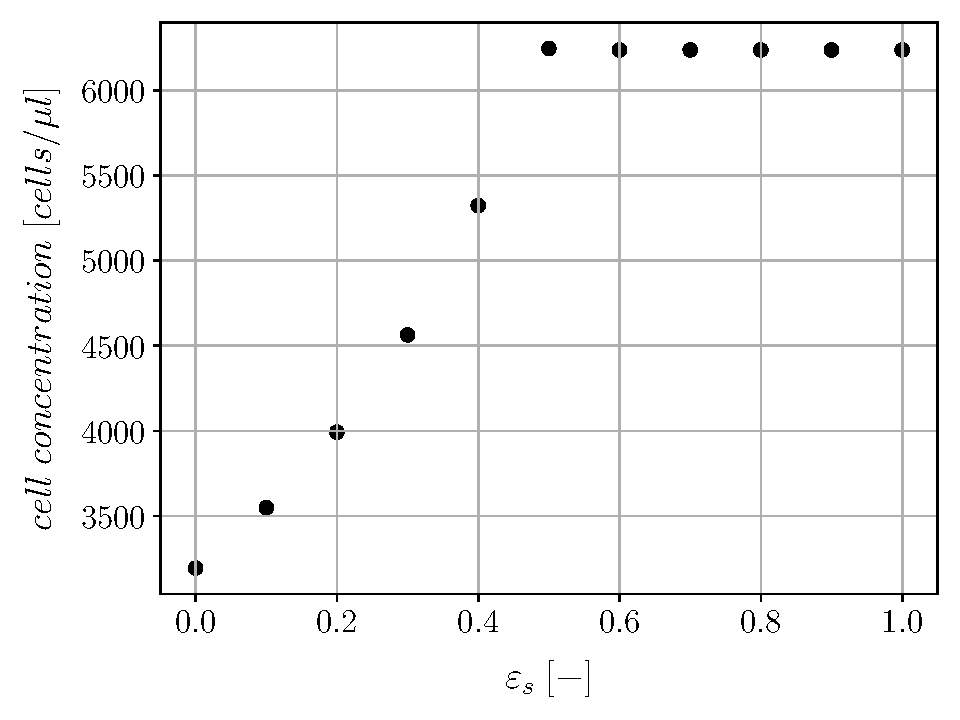
\includegraphics[width=\textwidth]{images/evolution_over_epsilon/treated_T.pdf}
        \caption[]%
        {{\small Uninfected CD4+ T cells}}    
        \label{fig3a:uninfected_T_cells}
    \end{subfigure}
    % \hfill
    % \begin{subfigure}[b]{0.3\textwidth}  
    %     \centering 
    %     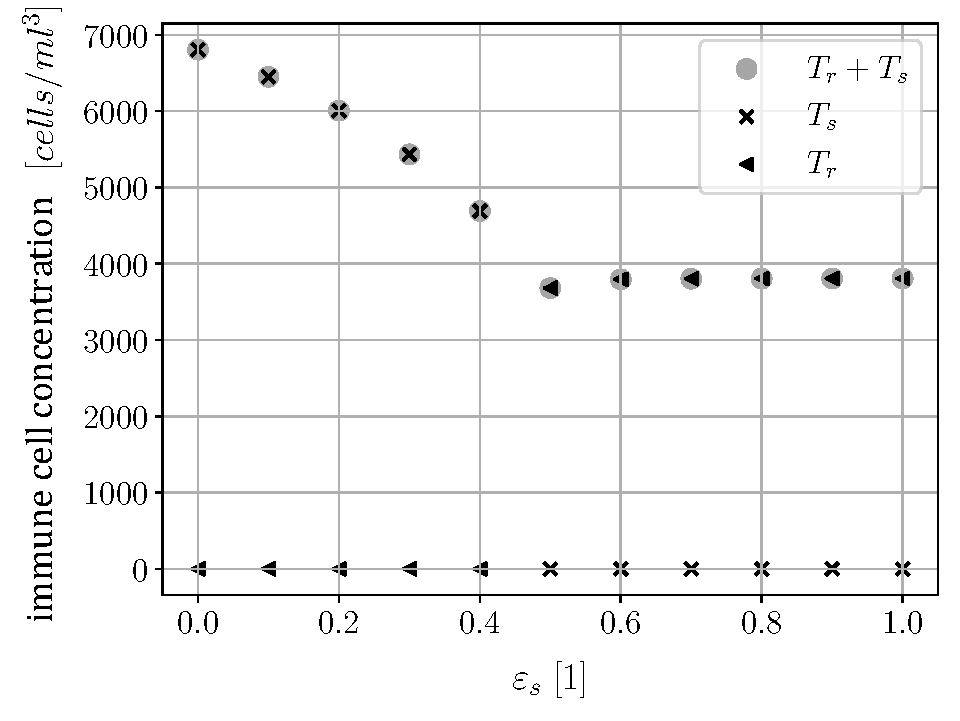
\includegraphics[width=\textwidth]{images/evolution_over_epsilon/treated_overview_infected_T.pdf}
    %     \caption[]%
    %     {{\small Infected CD4+ T cells}}    
    %     \label{fig3b:infected_T_cells}
    % \end{subfigure}
    % \vskip\baselineskip
    \begin{subfigure}[b]{0.475\textwidth}   
        \centering 
        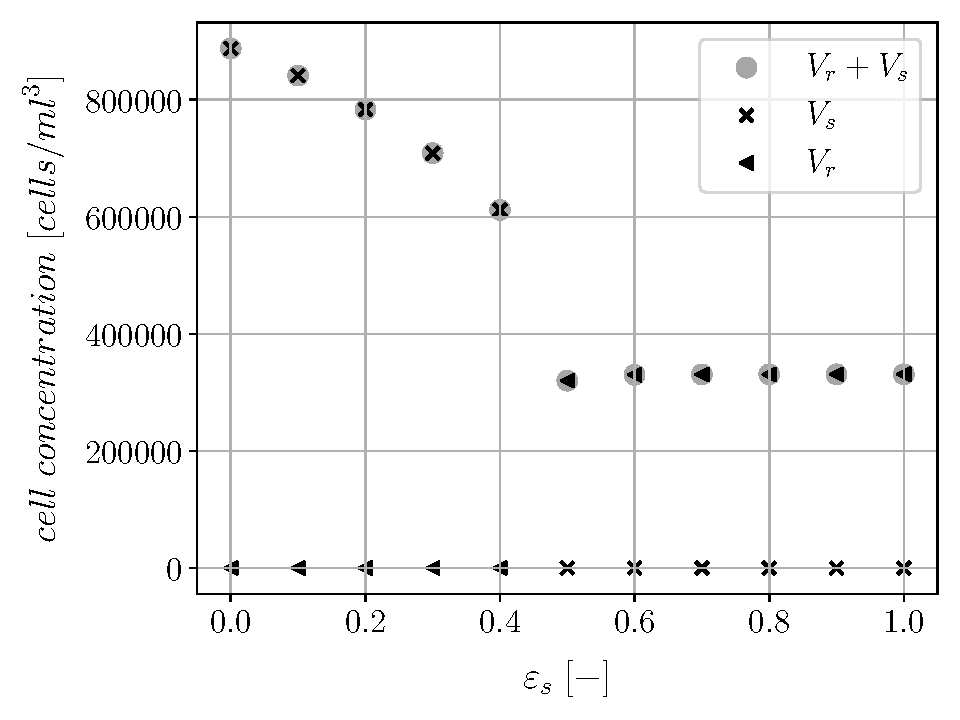
\includegraphics[width=\textwidth]{images/evolution_over_epsilon/treated_overview_V.pdf}
        \caption[]%
        {{\small Viral load}}    
        \label{fig3c:viral_load}
    \end{subfigure}
    \caption[]{The above diagrams show the dependency of the HIV infection on the drug efficacy parameter $\varepsilon_s$.
    In the considered case, it is $\varepsilon_{PI}^s =0$, $\varepsilon_{RT}^s = 0.4$ and $\alpha = 0.2$.
    Hence, the simulations basically demonstrate the impact of RTIs.
    Diagram (a) depicts the evolution of the immune cells over increasing $\varepsilon_s$. 
    Diagram (b) shows the same for the concentration of the viral strains.
    Although, initially enhancing the medication leads to a sinking viral cell count and hence, to a growing CD4+ T concentration, this behaviour changes for a sufficiently high $\varepsilon_s$.
    Above a certain threshold, the viremia is dominated by drug-resistant HIV cells. The patient does not longer respond to the therapy and her or his count of uninfcted immune cells remain constant under increasing $\varepsilon_s$.}
    \label{fig3:evolution_over_epsilon}
\end{figure}

\subsection{The Optimal Control Problem}
\label{subsec:Model_OptControl}

An optimal therapy is one, that maximizes the level of CD4+ T cells while deploying as few medication as possible.
Here, we assume that more and stronger drugs, i.e. higher $\varepsilon_s$ and $\varepsilon_r$, are associated with heavier 
side effects. 
Further, as shown in the preceding subsection \ref{subsec:Model_DynModel}, above a certain threshold efficacy $\varepsilon_{s,max}$, the effects of 
HAART saturate.\newline
From mathematical point of view, finding an ideal therapy can be formulated as an optimal control problem.
For this, we quantifiy the cost of HAART in the time interval $[t_0,t_1]$, by the functional

\begin{align}
    J(\mathbf{\varepsilon}) = \int_{t_0}^{t_1} \left(T^2(t) - A_1 \varepsilon_{s}^2 - A_2 \varepsilon_{r}^2\right) dt .
    \label{equ:cost_function}
\end{align}

The above relation has the following interpretation. 
The positive effect of the therapy, represented by the number of uninfected CD4+ T cells, is reduced by the negative side-effects of the drugs.
This medication burden is quantified by the product of the control parameters $\mathbf{\varepsilon} = (\varepsilon_s, \varepsilon_r)^T \in [0,1]^2$ and their weight constants $A_1$ and $A_2$ \cite{adams2005hiv,wu2010game}.
Ideally, $T(t)$ is maximised while $A_1 \varepsilon_{s}^2 + A_2 \varepsilon_{r}^2$ is minimized.
Hence, we seek an optimal control $\mathbf{\varepsilon}_{opt}$, such that

\begin{align}
    \mathbf{\varepsilon}_{opt} = \underset{\mathbf{\varepsilon} \in [0,1]^2}{\arg\max}\, (J(\mathbf{\varepsilon}_{opt})) \text{.}
    \label{equ:opti_control}
\end{align}
